\section{Processes within a Bureaucracy}

Processes are designed to limit bad behavior or to allocate scarce resources

Process friction, especially two uncoordinated processes, results in either exceptions to the process or lying or change in process. 
Example: receipts from on process submitted for reimbursement to another process.
Submitting the receipt shifts the accountability and justification burden to the accepting bureaucrat.


\href{https://en.wikipedia.org/wiki/Tragedy_of_the_commons}{Tragedy of the Commons} says that when there is a shared resource, someone will try to get away with behavior that is harmful to the organization.
Create processes for oversight/review/approval
Each process may be justifiable, but the aggregate is unreasonably burdensome


Deployment of processes and products need to account for 
normal users, Power users, malicious users, and edge cases



Processes with fewer people and fewer steps can be quicker and use fewer resources, but they are more fragile and less representative. Having more people involved helps with edge cases, but slows down the process. 

Any Nash equilibrium is constantly being upset by the change in conditions and change in people (who have varying motives).


    Processes can be undocumented. Then oral folklore is the mechanism. 
    
    Processes guardrails to prevent harm and keep stakeholders informed. 
    
    Without oversight processes, \href{https://en.wikipedia.org/wiki/Tragedy_of_the_commons}{tragedy of commons} occurs and malicious actors dominate.
    


\begin{figure}
    \centering
    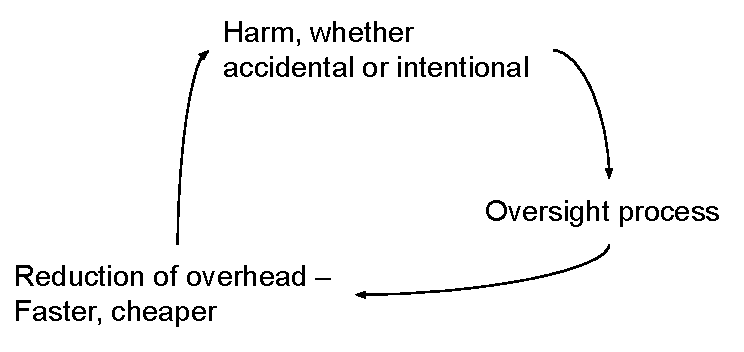
\includegraphics{images/process_loop_harm-oversight-improvement}
    \caption{loop: harm-oversight-improvement}
    \label{fig:harm-oversight-improvement}
\end{figure}


